\documentclass[a4paper,12pt]{article}
\usepackage[T2A]{fontenc}
\usepackage[utf8]{inputenc}
\usepackage[english,russian]{babel}
\usepackage{circuitikz}
\usepackage{wrapfig}
\usepackage{makecell}
\usepackage{pbox}
\usepackage{tabularx}
\usepackage{graphicx}
\usepackage{listings}

\parindent=0ex

\usepackage{cancel}
\usepackage{amsmath,amsfonts,amssymb,amsthm,mathtools}
\usepackage{tikz}
\usetikzlibrary{intersections}
\usetikzlibrary{arrows.meta}
\usetikzlibrary{calc,angles,positioning}
\usepackage{float}
\graphicspath{ {C:/Users/George/Documents/MIPT_TEX/LAB_1_2_2} }

\lstdefinestyle{mystyle}{
	backgroundcolor=\color{backcolour}, commentstyle=\color{codegreen},
	keywordstyle=\color{magenta},
	numberstyle=\tiny\color{codegray},
	stringstyle=\color{codepurple},
	basicstyle=\ttfamily\footnotesize,
	breakatwhitespace=false,         
	breaklines=true,                 
	captionpos=b,                    
	keepspaces=true,                 
	numbers=left,                    
	numbersep=5pt,                  
	showspaces=false,                
	showstringspaces=false,
	showtabs=false,                  
	tabsize=2
}
%New colors defined below
\definecolor{codegreen}{rgb}{0,0.6,0}
\definecolor{codegray}{rgb}{0.5,0.5,0.5}
\definecolor{codepurple}{rgb}{0.58,0,0.82}
\definecolor{backcolour}{rgb}{0.95,0.95,0.92}
\lstset{style=mystyle}

\begin{document}
	
	\begin{center}
		МОСКОВСКИЙ ФИЗИКО-ТЕХНИЧЕСКИЙ ИНСТИТУТ (НАЦИОНАЛЬНЫЙ ИССЛЕДОВАТЕЛЬСКИЙ УНИВЕРСИТЕТ) \\
		
		
		\hfill \break
		Факультет обшей и прикладной физики\\
		\vspace{2.5cm}
		\large{\textbf{Отчёт по лабораторной работе 1.2.2 <<Проверка закона вращательного движения на примере крестообразного маятника Обербека>>}}\\
		\hfill \break
		\\
	\end{center}
	
	\vspace{5cm}
	
	\begin{flushright}
		Выполнил:\\
		Студент гр. Б02-304\\
		Головинов. Г.А.
	\end{flushright}
	
	\vfill
	
	
	\begin{center} Долгопрудный, 2023 \end{center}
	
	\thispagestyle{empty}
	\newpage
	
	\pagenumbering{arabic}
	
	\section{Аннотация}
	\paragraph{Цель работы:} \hspace{-2mm} Проверить справедливость основного уравнения вращательного движения тела вокруг закреплённой оси, получив зависимость углового ускорения от момента инерции тела и момента сил, прикладываемых к системе тел, проанализировать влияние сил.
	\paragraph{Используемые инструменты:} \hspace{-2mm} Крестообразный маятник Обербека (Рис. 1), весы, штангенциркуль, компьютер с программой <<Kinetic>>, грузы различной массы. 
	\section{Основные теоретические сведения}
	\begin{figure}[H]
		\vspace{0mm}
		\centering
		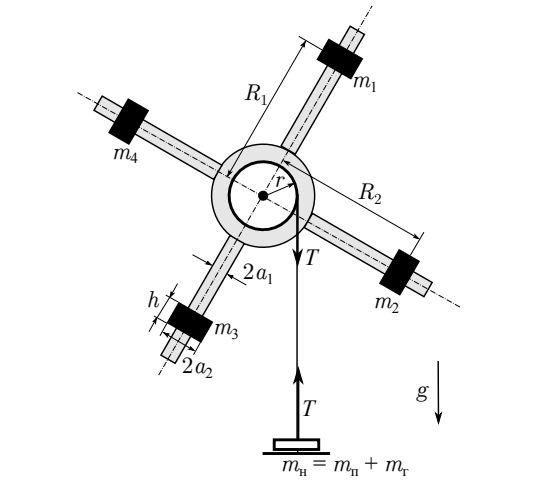
\includegraphics[width=0.75\linewidth,angle=0]{pend.png} 
		\caption{Крестообразный маятник Обербека}
		\label{fig:1}
	\end{figure}
	Основное уравнение вращательного движения:
	\begin{equation}
		\label{eq:1}
		I\varepsilon=M
	\end{equation}
	где $\varepsilon=\beta=\ddot{\varphi}$ -- угловое ускорение тела, $M$ -- суммарный момент всех сил, действующих на тело, $I$ -- момент инерции тела
	
	\paragraph{Некоторые необходимые в работе уравнения}\mbox{}\\
	Момент силы натяжения нити:
	$M_T=rT$, где $r$ -- радиус шкива.\\
	
	\noindent Сила $T$ выражается через $m_\text{н}\ddot{y}=m_\text{н}g-T$, где $m_\text{н}=m_\text{п}+m_\text{г}$ -- масса платформы с грузом\\
	
	\noindent Получим:
	\begin{equation}
		\label{eq:2}
		M_T=m_\text{н}r(g-\beta r)
	\end{equation} 
	
	\noindent Учитывая действие силы трения на маятник:
	\begin{equation}
		\label{eq:3}
		(I+m_\text{н}r^2)\beta=m_\text{н}gr-M_\text{тр}
	\end{equation}
	
	\noindent
	При проведении эксперимента получилось, что массы подвеса достаточно для медленного и равномерного вращения маятника. Это говорит, что $M_0<m_\text{п}gr=0,001545$ Н$\cdot$м
	
	\section{Результаты измерений и обработка данных}
	\paragraph{Рассчет момента инерции $I$ маятника через график $\beta_0(M_T)$:}
	Проводим 8 измерений с грузом $m=100$ г, чтобы получить случайную погрешность измерений $\beta_0$:
	\begin{table}[H]
		\centering
		\label{table:1}
		\caption{Результаты измерения $k$ и $\beta_0$}
		\begin{tabular}{|c|c|c|c|}
			\hline
			$k$, Гц & $\sigma_k$ &  $\beta_0$, рад/c$^2$ & $\sigma_{\beta_0}$ \\
			\hline
			-0,009043 & 0,00062 & 0,6165 & 0,00088 \\
			\hline
			-0,008601 & 0,00094 & 0,6163 & 0,00130 \\
			\hline
			-0,00779 & 0,00096 & 0,6104 & 0,00140 \\
			\hline
			-0,007661 & 0,00051 & 0,6111 & 0,00053 \\
			\hline
			-0,009521 & 0,00051 & 0,6219 & 0,00044 \\
			\hline
			-0,008676 & 0,00073 & 0,6148 & 0,00082 \\
			\hline
		\end{tabular}
	\end{table}
	\noindent
	По этим результатам по методу $\chi^2$ получим:
	\begin{equation}
		\label{eq:4}
		\sigma_{\beta_0}^{rnd}=0,000282 \text{ рад/c$^2$}
	\end{equation}
	\noindent
	$\beta_0$ возьмем как среднее:
	\begin{equation}
		\label{eq:5}
		\langle \beta_0 \rangle = 0,615166 \text{ рад/c$^2$}
	\end{equation}
	\noindent
	Погрешность $M_T$ вычислять будем по формуле:
	\begin{equation}
		\label{eq:n}
		\sigma_M=\sqrt{\left(\frac{\sigma_m}{m}\right)^2+\left(\frac{\sigma_g}{g}\right)^2}
	\end{equation}
	
	\noindent
	Погрешность измерения штангенциркуля $\sigma_r$ не будем учитывать, так как она много меньше измеренного радиуса шкива $r$, $\sigma_m$=0,5 г, $\sigma_g=0,01$.\\

	\begin{table}
		\centering
		\caption{Результаты $M_T$ по формуле \eqref{eq:2}}
		\small
		\begin{tabular}{|c|c|c|c|c|c|c|c|}
			\hline
			$m$, г & $r$, см & $k$, Гц & $\sigma_k$, Гц & $\beta_0$, рад/с$^2$ & $\sigma_{\beta_0}$ & $M_T$, Н$\cdot$м & $\sigma_M$ Н$\cdot$м \\
			\hline
			71 & 1,75 & -0,00696 & 0,00046 & 0,39390 & 0,00042 & 0,012180 & 8,67E-5 \\
			\hline
			109 & 1,75 & -0,08549 & 0,00026 & 0,61517 & 0,00028 & 0,018692 & 8,78E-5 \\
			\hline
			171 & 1,75 & -0,01135 & 0,00071 & 0,98040 & 0,00110 & 0,029305 & 9,07E-5 \\
			\hline
			209 & 1,75 & -0,01227 & 0,00064 & 1,21100 & 0,00100 & 0,035803 & 9,31E-5 \\
			\hline
			209 & 0,9 & -0,01156 & 0,00067 & 0,64380 & 0,00130 & 0,018442 & 4,80E-5 \\
			\hline
			171 & 0,9 & -0,01052 & 0,00068 & 0,51980 & 0,00120 & 0,015090 & 4,67E-5 \\
			\hline
			109 & 0,9 & -0,00801 & 0,00065 & 0,31900 & 0,00100 & 0,009621 & 4,52E-5 \\
			\hline
			70 & 0,9 & -0,00742 & 0,00055 & 0,20220 & 0,00065 & 0,006179 & 4,46E-5 \\
			\hline
		\end{tabular}
	\end{table}
	
	\begin{figure}[H]
		\centering
		\caption{График зависимости $\beta_0(M_T)$}
		\label{fig:2}
		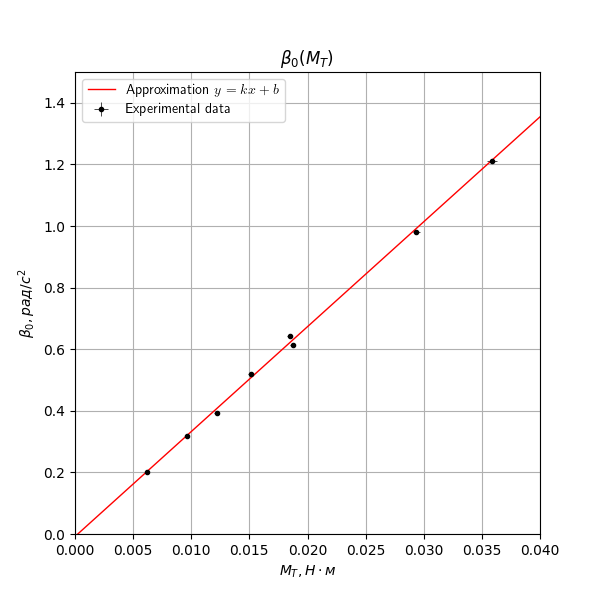
\includegraphics[width=0.7\linewidth]{fig_1}
	\end{figure}
	
	\newpage
	\begin{lstlisting}[language=Python,caption={Код построения графика и апроксимации по методу $\chi^2$}]
	import matplotlib.pyplot as plt
	import numpy as np
	from scipy.optimize import curve_fit
	plt.figure(figsize=(6, 6))
	plt.ylim(0,1.5)
	plt.xlim(0,0.04)
	plt.rcParams['text.usetex'] = True
	b0 = [0.3939, 0.615166, 0.9804, 1.211, 0.6438, 0.5198, 0.319, 0.2022]
	mt = [0.012189, 0.018713, 0.029356, 0.03588, 0.018453, 0.015098, 0.009624, 0.00618]
	sigmab0 = [0.00042, 0.000282, 0.0011, 0.001, 0.0013, 0.0012, 0.001, 0.00065]
	sigmam = [0.0002, 0.0002, 0.0003, 0.0004, 0.0002, 0.0002, 0.0001, 0.0001]
	
	f = lambda k,x,b: k*x+b
	popt,pcov = curve_fit(f,mt,b0,sigma=sigmam)
	k,b = popt
	print(1/k,b)
	pp = []
	p1 = plt.errorbar(mt,b0,sigmam,sigmab0,fmt='.k',elinewidth=0.5,label=r"Experimental data")
	z = np.poly1d (np.polyfit(mt,b0,1))
	x=np.linspace(0,0.04,100)
	plt.plot(x,f(k,x,b),'r-',linewidth=1,label=r"Approximation $y=kx+b$")
	print(-b/k)
	
	plt.title(r'$\beta_0(M_T)$')
	plt.legend(loc='upper left')
	plt.grid()
	plt.show()
	\end{lstlisting}
	\newpage
	
	\noindent
	Видно, что экспериментальные точки довольно хорошо ложаться на прямую, что подтверждает справедливость основного уравнения вращательного движения.\\
	
	При аппроксимации через метод $\chi^2$ получаем прямую $y=kx+b$, где $k=34,1325$, $b=-0,0086$. Все экспериментальные точки хорошо ложатся на прямую, что соответствует теории.\\
	
	\noindent
	Пересечение с осью абсцисс при $M_0=0,00023792$ Н$\cdot$м, что действительно много меньше $m_\text{п}gr$, значит полученные данные соотносятся с наблюдением.\\
	
	\noindent
	Определим момент инерции с помощью коэффициента наклона $k=I^{-1}\Rightarrow I=0,029357$ кг$\cdot$м$^2$, а погрешность составила $\sigma_I=0,017782$
	
	\[
	I=(0,029357\pm 0,000239) \hspace{1mm} \text{кг}\cdot\text{м}^2
	\]
	
	Погрешность составила около $1\%$ (почему так -- обсудим в выводах)
	
	\paragraph{Рассчет момента инерции $I$ вторым способом}
	Зная массы грузов, их расстояния до оси вращения, их внешний и внутренний радиус мы можем рассчитать момент инерции системы маятник-грузы следующим образом:
	\begin{equation}
		\label{eq:7}
		I=I_0+\sum_{i=1}^4(I_i+m_iR_i^2)
	\end{equation}
	где $I_0$ -- момент инерции маятника без грузов, а
	\begin{equation}
		\label{eq:8}
		I_i=\frac{1}{12}m_ih^2+\frac{1}{4}m_i(a_1^2+a_2^2)
	\end{equation}	
	
	Найдем $I_0$ по аналогии с маятником с грузами:
	
	\begin{table}[H]
		\centering
		\caption{Результаты измерения для маятника без грузов}
		\begin{tabular}{|c|c|c|c|c|c|}
			\hline
			$m$, г & $r$, см & $\beta_0$, рад/с$^2$ & $\sigma_{\beta_0}$, рад/с$^2$ & $M_T$, Н$\cdot$м & $\sigma_M$, Н$\cdot$м \\
			\hline
			53 & 0,9 & 1.592 & 0,0059 & 0,00467937 & 4,44E-05 \\
			\hline
			70 & 0,9 & 2,092 & 0,0100 & 0,00618030 & 4,46E-05 \\
			\hline
			109 & 0,9 & 3,298 & 0,0093 & 0,00962361 & 4,52E-05 \\
			\hline
			170 & 0,9 & 5,187 & 0,0120 & 0,01500930 & 4,67E-05 \\
			\hline
			209 & 0,9 & 6,533 & 0,0200 & 0,01845261 & 4,80E-05 \\
			\hline
		\end{tabular}
	\end{table}
	
	\begin{figure}[H]
		\centering
		\caption{Зависимость $\beta_0(M_T)$ для маятника без грузов}
		\label{fig:fig2}
		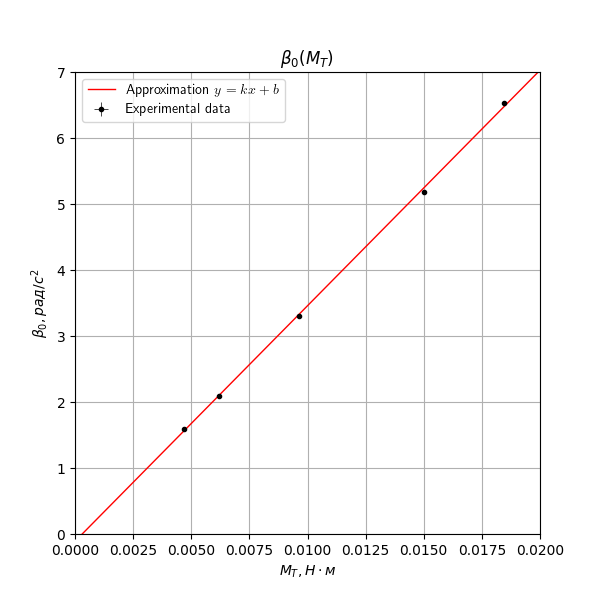
\includegraphics[width=0.9\linewidth]{fig_2}
	\end{figure}
	
	Получим
	\[
	I_0=(0,002801\pm 0,000148)  \hspace{1mm} \text{кг}\cdot\text{м}^2
	\] 
	Почему получилась такая погрешность -- обсудим в выводах
	
	\vspace{2mm}
	
	$I_i$ вычисляем по формуле \eqref{eq:8} и получаем
	\[
	\sum_{i=1}^4(I_i+m_iR_i^2)=0,0239  \hspace{1mm} \text{кг}\cdot\text{м}^2
	\]
	
	Погрешность в данном случае вычисляем по формуле:
	\begin{equation}
		\label{eq:9}
		\sigma_{\sum I}=I\sqrt{\left(\frac{\sigma_m}{m}\right)^2+\left(2\frac{\sigma R}{R}\right)^2}
	\end{equation}
	Погрешностью измерения $h, a_1, a_2$ пренебрегаем, так как они были измерены с помощью штангенциркуля, а $\sigma_R$ примем за 1 см.
	Итого получаем
	\[
	I_i=(0,0239\pm 0,0024)  \hspace{1mm} \text{кг}\cdot\text{м}^2
	\]
	А полный момент инерции получился
	\[
	I=(0,0267 \pm 0,0024) \hspace{1mm} \text{кг}\cdot\text{м}^2
	\]
	Получили значение момента инерции маятника двумя способами: с помощью графика $\beta_0(M_T)$ и с помощью теоретических соотношений (уравнения \eqref{eq:7} и \eqref{eq:8}). Они очень хорошо соотносятся (и даже почти попадают в интервал $\pm 1\sigma$)
	
	\subsection{Интересный колебательный процесс, который мы наблюдали во время выполнения работы}
	
	Изначально (несмотря на очень хорошую балансировку) нам не удавалось получить хорошие данные при измерении подъема и спуска груза, поэтому мы перешли в режим измерения спуска. Это улучшило ситуацию, однако в примерно половине случаев результаты имели явные колебания, которые не давали возможности доверять полученным значениям. Была выдвинута гипотеза -- на результаты влиял способ намотки нити (по часовой или против), что не имело никакого физического смысла, однако оказалось правдой. Мы измерили самые <<красивые>> колебания, чтобы потом их нанести на график и вот что из этого получилось:
	
	\begin{figure}[H]
		\centering
		\caption{Результаты измерений при <<неправильной>> намотке нити}
		\label{fig:fig3}
		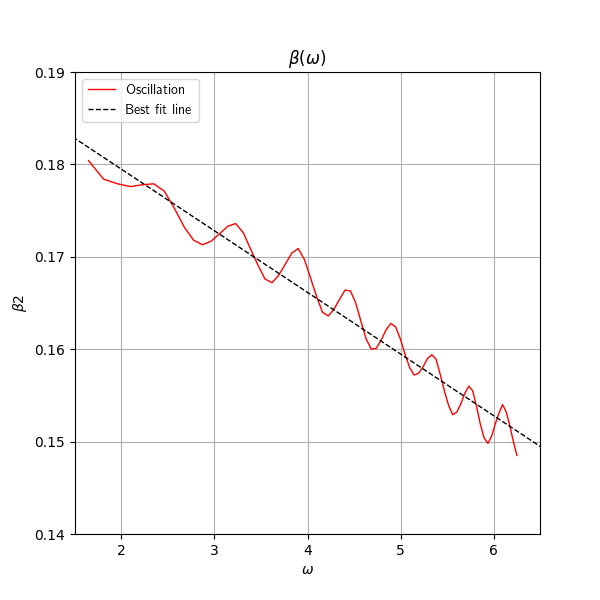
\includegraphics[width=0.65\linewidth]{fig_3}
	\end{figure}
	
	\begin{figure}[H]
		\centering
		\caption{Результаты измерений при <<неправильной>> намотке нити (с вычетом прямой по МНК)}
		\label{fig:fig4}
		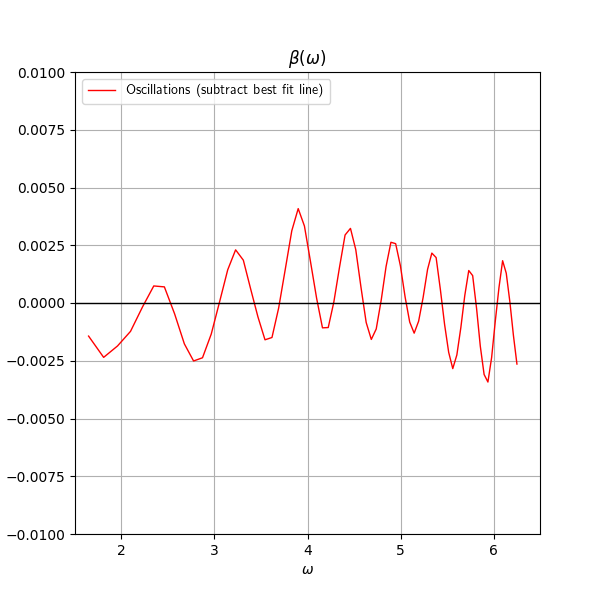
\includegraphics[width=0.65\linewidth]{fig_4}
	\end{figure}
	
	
	К сожалению, в установленное время не было возможности должным образом воспроизвести этот эффект после пересборки экспериментальной установки, поэтому эта часть работы требует продолжения и заключения.
	
	
	\section{Обсуждение результатов и выводы}
	
	В ходе работы мы проверили справедливость основного уравнения вращательного движения (рис. \ref{fig:2}) \\
	
	Также мы измерили момент инерции крестообразного маятника Обербека двумя способами: с помощью теоретических соотношений (уравнения \eqref{eq:7}-\eqref{eq:8}) и с помощью углового коэффициента зависимости $\beta_0(M_T)$\\
	
	Полученные этими двумя методами значения очень хорошо соотносятся и почти попадают в пределы $\pm 1\sigma$ друг от друга (относительная погрешность $\varepsilon=9,05\%$). Можно сказать, что погрешность измерений была недооценена, поэтому получилось, что данные расходятся друг от друга более чем на $\pm 1 \sigma$\\
	
\end{document}